\section{Introduction}
\label{sec:introduction}

% state the learning objective 

\hspace{0,5cm} This report is being made for the subject of Circuit Theory and Electronics Fundamentals and is related to the $2^{st}$ laboratory being its objective to study an RC circuit containing seven resistors, one sinusoidal voltage source, one capacitor, one current controlled voltage source and one voltage controlled current source. The four elementary meshes are named after the current to which they are attributed.

The current controlled voltage source $V_d$ is calculated by multiplying $K_d$ with the current $I_d$, whereas the voltage controlled current source $I_b$ can be determined by multiplying $K_b$ with the voltage source $V_b$.

The display of this circuit can be seen in Figure~\ref{fig:circuito}.

In Section~\ref{sec:analysis} the circuit will be analysed theoretically ATENÇÃO ending with the presentation of the results obtained by Octave.

Secondly, in Section~\ref{sec:simulation} it will be simulated the circuit using ngspice, the results obtained will be presented and 

Following with both results from Section~\ref{sec:analysis} and Section~\ref{sec:simulation} being compared and commented.

The conclusions of this study are outlined in Section~\ref{sec:conclusion}.

\begin{figure}[H] \centering
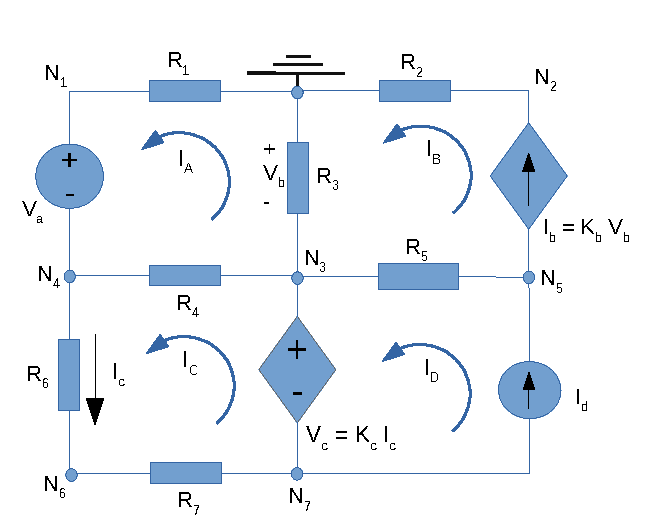
\includegraphics[width=1\linewidth]{circuito.pdf}
\caption{Circuit in analysis}
\label{fig:circuito}
\end{figure}

Where:
\begin{center}
\begin{table}[H]
 \centering
  \begin{tabular}{|c|c|}
    \hline    
    {\bf Name} & {\bf Value [A or V]} \\ \hline
    \input{../mat/data_tab}
  \end{tabular}
  \caption{Results obtained by mesh analysis method with octave}
  \label{tab:mesh}
\end{table}
\end{center}

MUDAR The units of the elements whose name starts with R (the resistors) are $k\Omega$ (kiloohm), the ones that start with I are expressed in $mA$ (miliampere) and the ones starting with V are expressed in $V$ (volts). While Kb is given in $mS$ (milisiemens), Kc is also given in $k\Omega$.

These values where obtained using the Python script using the lowest student number on our group - 95785.


